%% =====================================================================
%%  Significance filtering induces denominator selection bias in local
%%  genetic correlation
%%
%%  Submission to Genetic Epidemiology (Wiley), free-format submission.
%%  Build: pdflatex manuscript; pdflatex manuscript
%%  (references are embedded, no BibTeX run is needed)
%% =====================================================================
\documentclass[12pt,a4paper]{article}

\usepackage[T1]{fontenc}
\usepackage[utf8]{inputenc}
\usepackage{lmodern}
\usepackage[margin=2.54cm]{geometry}
\usepackage{amsmath,amssymb,bm}
\usepackage{booktabs}
\usepackage{array}
\usepackage{graphicx}
\usepackage{setspace}
\usepackage[switch,mathlines]{lineno}
\usepackage{caption}
\usepackage[authoryear,round,semicolon]{natbib}
\usepackage{url}
\usepackage[colorlinks=true,allcolors=black,urlcolor=blue,citecolor=black,linkcolor=black]{hyperref}

\captionsetup{font=small,labelfont=bf,labelsep=period,justification=raggedright,singlelinecheck=false}
\setcitestyle{aysep={,}}
\renewcommand{\bibsection}{\section*{References}}
\setlength{\bibhang}{1.27cm}
\urlstyle{same}

\graphicspath{{figures/}}

\newcommand{\rh}{\hat{\rho}}
\newcommand{\Om}{\bm{\Omega}}
\newcommand{\Sig}{\bm{\Sigma}}
\newcommand{\Slocus}{S_{\mathrm{loc}}}
\newcommand{\Ilocus}{I_{\mathrm{loc}}}
\newcommand{\re}{r_{\mathrm{e}}}
\newcommand{\crf}{c_{\mathrm{ref}}}
\newcommand{\Nref}{N_{\mathrm{ref}}}

\emergencystretch=2em
\tolerance=2000

\begin{document}

\linenumbers
\onehalfspacing

%% ------------------------------ Title page ---------------------------
\begin{titlepage}
\begin{singlespacing}
\begin{center}
{\LARGE\bfseries Significance filtering induces denominator selection bias in local genetic
correlation: closed-form characterization, a gate-aware correction, and an applicability
diagnostic\par}
\vspace{1.2cm}
{\large Dana Paquin$^{1,*}$ and Riddhiman Jain$^{2}$\par}
\vspace{0.6cm}
{\small
$^{1}$Stanford University, Stanford, California, USA\\
$^{2}$Independent Researcher, Ahmedabad, India\\[6pt]
$^{*}$Corresponding author: Dana Paquin, \href{mailto:dpaquin@stanford.edu}{dpaquin@stanford.edu}\par}
\end{center}
\vspace{0.8cm}

\noindent\textbf{Running title:} Selection bias in local genetic correlation

\medskip
\noindent\textbf{Data availability statement.} All analysis code, the correction module and
every result file underlying a number in this paper are openly available in Zenodo at
\url{https://doi.org/10.5281/zenodo.22830134} (version used here) and
\url{https://doi.org/10.5281/zenodo.22132758} (all versions), and on GitHub at
\url{https://github.com/riddhimanjain/lava-gate}. The GWAS summary statistics analyzed are
publicly available from the Psychiatric Genomics Consortium; see the Data and code
availability section.

\medskip
\noindent\textbf{Funding statement.} This work received no funding from any agency in the
public, commercial or not-for-profit sectors.

\medskip
\noindent\textbf{Conflict of interest disclosure.} The authors declare no competing interests.

\medskip
\noindent\textbf{Ethics approval statement.} This study analyzed only previously published,
publicly available aggregate GWAS summary statistics. No individual-level data were
accessed and no new participants were recruited, so no ethics approval was required.

\medskip
\noindent\textbf{Patient consent statement.} Not applicable.

\medskip
\noindent\textbf{Permission to reproduce material from other sources.} Not applicable.

\medskip
\noindent\textbf{Clinical trial registration.} Not applicable.
\end{singlespacing}
\end{titlepage}

%% ------------------------------- Abstract ----------------------------
\section*{Abstract}

Local genetic correlation is the ratio of a local genetic covariance to the geometric mean
of two local heritabilities. LAVA, the standard implementation, reports it only where both
traits pass a univariate heritability test at $P<0.05$, a rule presented as a stabilizer. We
show that the rule is a selection event acting on the denominator. Under the noncentral
Wishart model that LAVA's own interval routine assumes, the gate-conditional mean of the
estimator is affine in the true correlation, with closed-form slope and intercept computable
from quantities every run reports. Across six psychiatric trait pairs the measured slope
ranges from 0.579 to 0.923 and the closed form predicts each within 0.007, with nothing
fitted; within one pair it ranges from 0.371 to 0.971, so no single factor can correct it.
Sample overlap and the filter jointly manufacture correlation where the truth is zero. A
gate-aware correction reduces mean absolute bias from 0.247 to 0.026 over 48 simulation
cells, and a diagnostic determines whether correction is identified; three pairs sharing one
trait fail it.

\medskip
\noindent\textbf{Keywords:} local genetic correlation; LAVA; selection bias; ratio
estimator; sample overlap; bias correction; statistical genetics

\clearpage

\section{Introduction}\label{sec:intro}

Genome-wide genetic correlation compresses the shared genetic basis of two traits into one
number, averaging over regions that may not agree. Local methods were built to recover
that structure, and LAVA \citep{ref1} has become the standard tool which partitions the
genome into approximately independent linkage-disequilibrium blocks and estimates a
genetic correlation within each. Local estimates are now read as biological findings in
their own right, particularly in psychiatric genetics \citep{ref2}, where the question
asked of them is usually about the sign of the relationship in a named region.

The estimand is a ratio that is prone to error. Its denominator is the geometric mean of
the two local heritabilities, each small, noisily estimated within a single block, and
free to go negative. LAVA handles this by reporting the correlation only where both traits
clear a univariate heritability test at $P<0.05$. LAVA's documentation describes this as a
way to filter out non-associated loci that may yield unstable correlation estimates.

Specifically, what it does is not benign. The univariate statistic and the denominator are
built from the same sum of squares, so conditioning on the statistic being large conditions
on the denominator being large. Among loci sharing a true local heritability, those
admitted are disproportionately those at which sampling noise inflated the estimate, and an
inflated denominator shrinks a ratio. This selection may look comparable to the winner's
curse, but the two differ in several ways. The winner's curse selects on the estimand and
inflates it \citep{ref3,ref4}. Here selection acts on the denominator, so the bias
attenuates rather than inflates. It is affine in the true correlation rather than a
threshold-dependent shift, and it interacts with sample overlap to produce non-zero
expected correlation even where the truth is zero, which the winner's curse does not.

Benchmarking work has compared local genetic correlation methods for accuracy and power
under a common truth \citep{ref5}. The selection induced by a method's own reporting rule
has not been characterized. We do that here, and supply a correction that inverts the
characterization with a validation of it against LAVA's own code path on real loci, and a
diagnostic that states exactly where the correction works. We then run the protocol across
six trait pairs spanning the two dimensions along which the bias varies, that is, the
weaker trait's power and the overlap between the two GWAS. That survey is about how the
method behaves in the regimes practitioners work in, but does not indicate or conclude
anything concrete about the biology of any disorder pair.

%% =====================================================================
\section{Methods}\label{sec:methods}
%% =====================================================================

\subsection{The estimator, and the gate as implemented}\label{sec:estimator}

We work from the actual LAVA source, version 0.1.5, not from its description, and state the
file and line for each anomaly or inconsistency we find. Table~\ref{tab:notation} fixes
notation.

For a locus retaining $K$ principal components of the local LD matrix and two traits,
we let $\bm{\delta}$ be the $K\times2$ matrix of joint effect estimates in
principal-component space, with rows drawn independently as
$\bm{d}_k\sim N(\bm{\mu}_k,\Sig)$, the off-diagonal of $\Sig$ carrying the sample
overlap $\re$. Writing $\bm{S}=\bm{\delta}'\bm{\delta}$, LAVA forms the bias-corrected
local genetic covariance matrix as $\hat{\Om}=(\bm{S}/K-\Sig)\,\crf$ with
$\crf=(\Nref-K-1)/(\Nref-1)$ (\texttt{input\_processing.R:134--166}), and the local
genetic correlation as $\rh=\hat\Omega_{12}/\sqrt{\hat\Omega_{11}\hat\Omega_{22}}$, in
which $\crf$ cancels. For binary traits the univariate statistic is
$U_i=(S_{ii}/\Sigma_{ii})\,\crf$, referred to $\chi^2_K$. Liability-scale heritabilities
are obtained afterwards \citep{ref15} and play no part in the gate, which is evaluated on
$\bm{\delta}$ and $\Sig$ directly. In v0.1.5 $\crf$ evaluates to
exactly 1, because \texttt{nref.correction} is assigned \texttt{FALSE} inside
\texttt{process.locus()} and is not exposed to the caller.

Define $\theta_i=\Omega_{ii}/\Sigma_{ii}$, the local signal-to-noise ratio. Since $\Sig$
scales as $1/N$, $\theta_i$ is proportional to sample size, and the univariate
noncentrality is $K\theta_i$, so a locus is well powered either by carrying much signal or
by retaining many components. The gate is $U_1>\chi^2_{K,\,0.95}$ and
$U_2>\chi^2_{K,\,0.95}$ (\texttt{analysis\_functions.R:42--44}). Everything below is
derived for the $\chi^2$ case and so applies to binary traits only.

\medskip
\noindent\textbf{The filter and the denominator are not separable.} Because
$\hat\Omega_{ii}=\Sigma_{ii}(U_i/K-\crf)$ with $\crf=1$, the sign of the estimated local
heritability is fixed by whether $U_i$ exceeds $K$, and the 5\% critical value of a
$\chi^2_K$ exceeds $K$ for every $K$. Because passing the gate implies
$\hat\Omega_{ii}>0$ for both traits, the gate is a strict subset of the set on which
$\rh$ is defined at all. There is no configuration in which the filter is inactive and
the estimator remains well posed, so ``what LAVA would report without the filter'' is
not a quantity the software can produce. This determines how the attenuation must be
measured, and we verify it (Section~\ref{sec:tiers}).

\begin{table}[htbp]
\caption{Notation.}\label{tab:notation}
\small
\begin{center}
\resizebox{\textwidth}{!}{%
\begin{tabular}{@{}lll@{}}
\toprule
Symbol & Meaning & Source \\
\midrule
$K$ & principal components retained at the locus & \texttt{process.locus()\$K} \\
$\bm{\delta}$ & $K\times2$ matrix of joint effects in PC space & internal \\
$\bm{S}=\bm{\delta}'\bm{\delta}$ & sums of squares and cross-products & internal \\
$\Sig$ & residual covariance; off-diagonal carries overlap & internal \\
$\Om,\hat{\Om}$ & true and estimated local genetic covariance & \texttt{locus\$omega} \\
$\rho,\rh$ & true and reported local genetic correlation & \texttt{run.bivar()\$rho} \\
$\re$ & sample-overlap correlation between the two GWAS & cross-trait LDSC \\
$\theta_i=\Omega_{ii}/\Sigma_{ii}$ & local signal-to-noise ratio & recovered from $P_i$ \\
$U_i$ & univariate statistic, referred to $\chi^2_K$ & implied by \texttt{run.univ()\$p} \\
$G$ & the gate: both traits clear $P<0.05$ & \texttt{analysis\_functions.R:42--44} \\
$\Delta_i$ & gate-induced inflation of $S_{ii}$ & closed form, \S\ref{sec:closedform} \\
$d_i=\theta_i+\Delta_i/K$ & gated local heritability, on the $\theta$ scale & observed \\
$g_K$ & map from $\theta$ to its gated expectation & inverted in Stage 1 \\
$\Slocus,\Ilocus$ & per-locus attenuation slope and manufactured intercept & closed form \\
$\Nref$ & LD reference sample size (99,339) & LAVA v1.1 panel \\
$\crf$ & reference-size correction; equals 1 in v0.1.5 & \texttt{locus\$nref.scale} \\
\bottomrule
\end{tabular}}
\end{center}
\end{table}

\subsection{Where loci and phenotypes are lost}\label{sec:attrition}

Tracing each loss on real data to its source identifies five distinct mechanisms, two of
which are wholly undocumented and one partially (Supplementary Table~S1). The consequential
one is Channel~2: when a trait's local variance estimate goes negative,
\texttt{input\_processing.R:169--171} silently removes that trait and returns the locus as
if analyzable. Analysis code assuming both phenotypes are present will therefore evaluate
the gate on whichever trait survived and produce a well-formed result for a comparison that
was never made, and because the trigger is a negative variance estimate the mechanism
preferentially removes the weaker trait. Parsing every warning across the panel confirms
the documented trigger and no second pathway: 1,407 of 1,407 drops for P3 and 1,474 of
1,474 for P5 carry a negative-variance warning. A second mechanism shows how far the
filter is load-bearing: \texttt{run.bivar()} raises an error and halts on a locus it cannot
analyze, and users never meet this only because the gate guarantees the positive
denominator it needs.

\begin{figure}[htbp]
\begin{center}
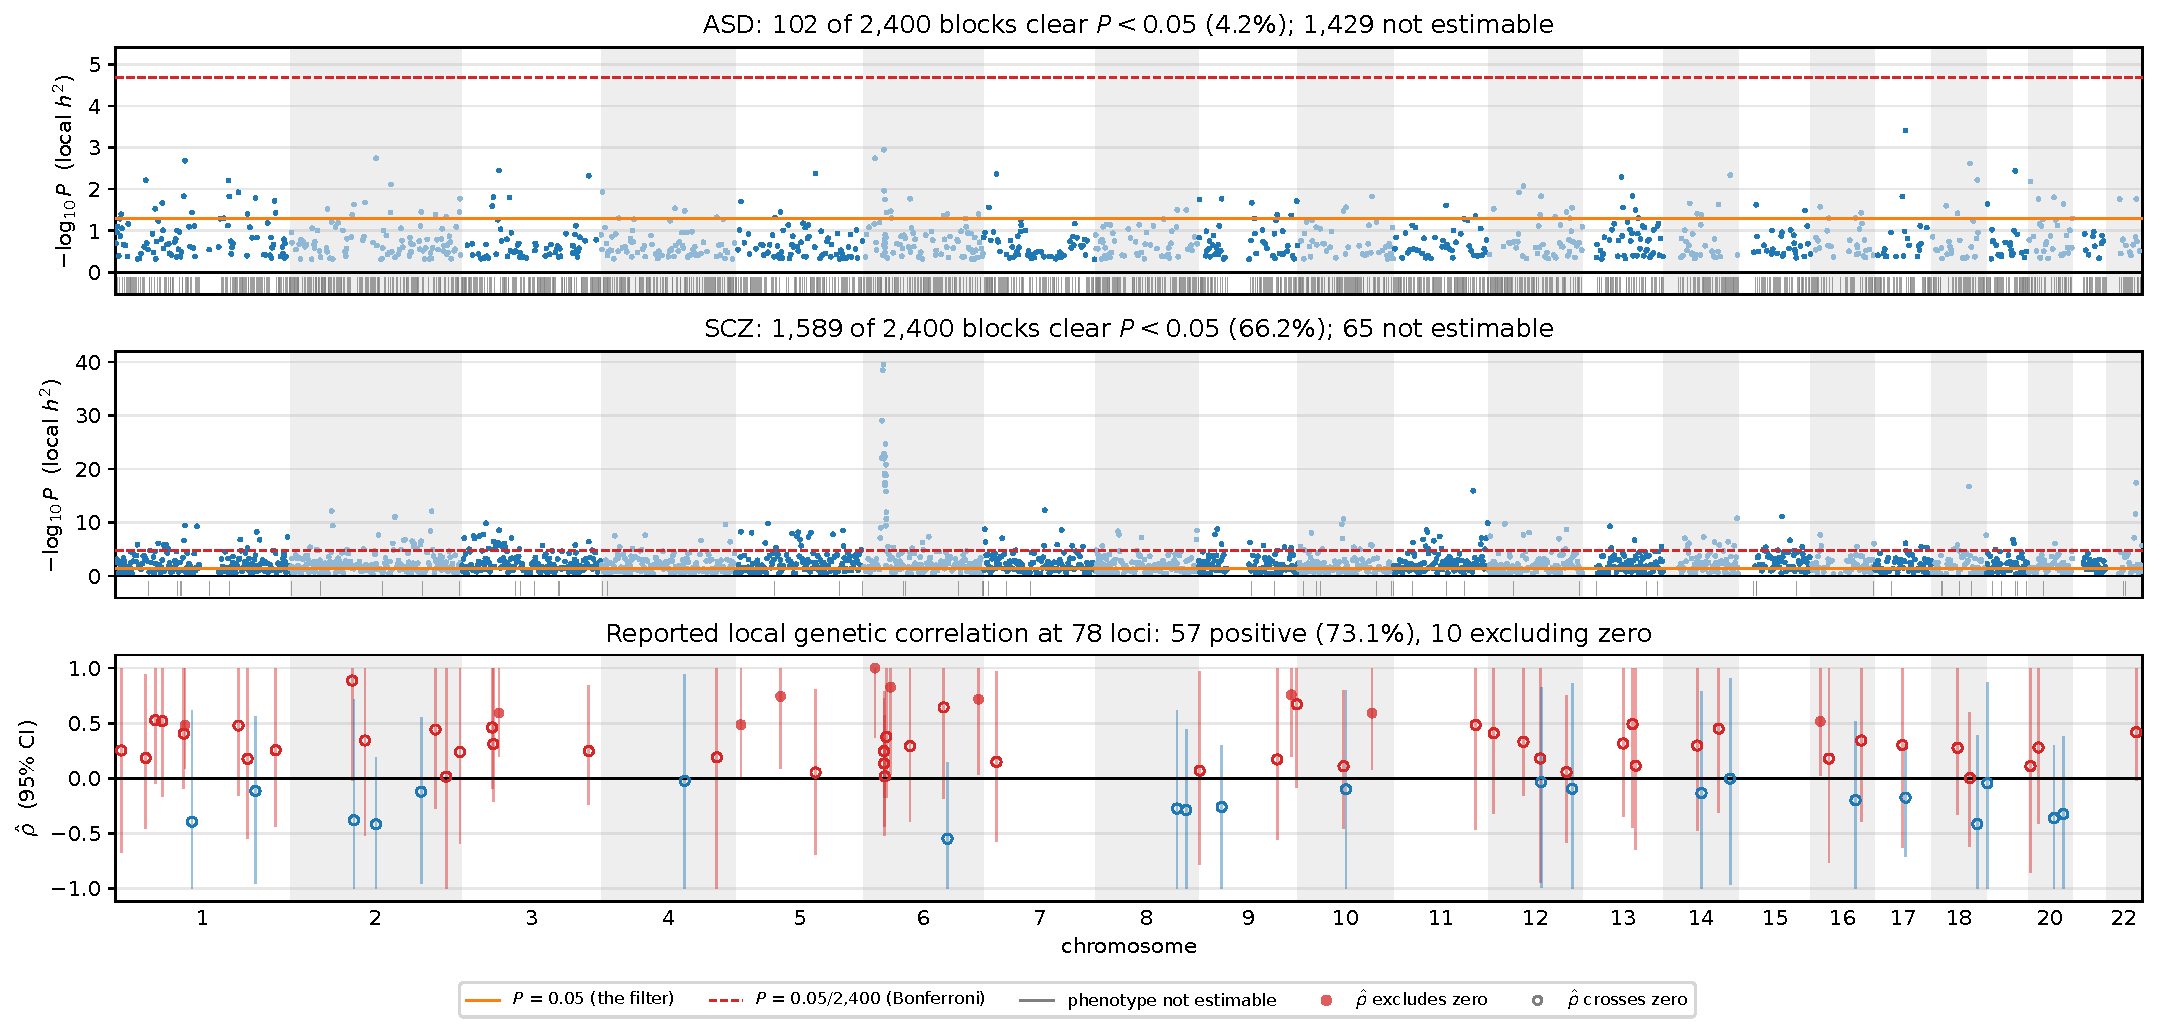
\includegraphics[width=0.95\textwidth]{Figure1_genomewide.pdf}
\caption{\textbf{The univariate filter applied across the genome, on P4 (ASD $\times$ SCZ).} Univariate local-heritability significance for each trait across the 2,400 processed blocks, with LAVA's filter and the Bonferroni threshold marked, and the 78 blocks at which both traits clear the filter. Ticks below each baseline mark blocks silently dropped by Channel~2.}
\label{fig:1}
\end{center}
\end{figure}

\subsection{The gate-conditional mean, in closed form}\label{sec:closedform}

$\bm{S}$ follows a noncentral Wishart, $\bm{S}\sim W_2(K,\Sig,\bm{\Theta})$, as confirmed
by LAVA's own interval routine, which draws from
\texttt{rwishart(n.iter, K, Sigma = sigma/K, Theta = omega)}. The derivation rests on two
identities that remove any need for quadrature: a noncentral $\chi^2$ is a
Poisson-weighted mixture of central ones, and the truncated first moment of a central
$\chi^2$ is $E[\chi^2_m\mathbf{1}\{\chi^2_m>t\}]=m\,P(\chi^2_{m+2}>t)$. Together they give
the gate pass probability and the truncated first moment of $S_{ii}$ exactly
(Supplementary Methods S1). Define $\Delta_i=E[S_{ii}\mid S_{ii}>t]-E[S_{ii}]$, the
gate-induced inflation of the $i$th diagonal.

Treating the numerator as unaffected gives the leading-order account, attenuation
$=1/\sqrt{a_1a_2}$ with $a_i$ the conditional heritability inflation. We pre-specified
that prediction and it was falsified. Simulated slopes exceed it by 8--33\%. The gate
inflates the numerator too, because $S_{12}$ shares noise with $S_{11}$ and $S_{22}$.
Linearizing $S_{12}$ on the two diagonals through the exact noncentral Wishart covariance,
$\mathrm{Cov}(S_{12},S_{11})=2K(\re+\Omega_{12}+\re\Omega_{11})$ and
$\mathrm{Var}(S_{11})=2K(1+2\Omega_{11})$, gives weights
$b_i=(\re+\Omega_{12}+\re\theta_i)/(1+2\theta_i)$ and
\begin{equation}
E[\rh\mid G] \approx
\frac{\Omega_{12}+\bigl(b_1\Delta_1+b_2\Delta_2\bigr)/K}{\sqrt{d_1d_2}},
\qquad d_i=\theta_i+\frac{\Delta_i}{K}.
\end{equation}

Each $b_i$ is affine in $\Omega_{12}$, and
$\Omega_{12}=\rho\sqrt{\theta_1\theta_2}$ is linear in $\rho$, while $\Delta_i$ and $d_i$
do not depend on $\rho$ at all: the gate is a condition on the diagonals only, and their
conditional moments are functions of $\theta_i$ and $K$. The expression is therefore
affine in $\rho$ exactly rather than to leading order,
$E[\rh\mid G]=\Slocus\rho+\Ilocus$, with
\begin{equation}
\begin{aligned}
\Slocus &= \frac{\sqrt{\theta_1\theta_2}}{\sqrt{d_1d_2}}
  \Bigl(1+\frac{1}{K}\sum_i \frac{\Delta_i}{1+2\theta_i}\Bigr),\\[2pt]
\Ilocus &= \frac{\re}{K\sqrt{d_1d_2}}
  \sum_i \frac{\Delta_i(1+\theta_i)}{1+2\theta_i}.
\end{aligned}
\end{equation}

Affinity in $\rho$ is algebraic rather than an expansion, that is, no term in $\rho^2$ is
dropped because none is generated, and two approximations sit behind it. The
linearization replaces $E[S_{12}\mid S_{11},S_{22}]$ by its least-squares linear predictor,
exact for a Gaussian pair and approximate for a noncentral Wishart. And $\Delta_i$ is the
inflation induced by each trait's own gate, whereas the gate conditions on both diagonals
at once: these are dependent whenever $\re\neq0$, with
$\mathrm{Cov}(S_{11},S_{22})=2K(\re^2+2\re\Omega_{12})$, which itself carries $\rho$. That
dependence vanishes at $\re=0$ and is second order in $\re$ elsewhere, so the residual
inaccuracy is carried almost entirely by the values of $\Slocus$ and $\Ilocus$ rather than
by the shape. Adding a quadratic term to the pooled Tier~B fit does not improve it
($P=0.936$, Section~\ref{sec:attrib}), which bounds the departure empirically.

Two features do the work later. $d_i$ is exactly the gated local heritability LAVA already
reports, so the denominator $\sqrt{d_1d_2}$ is observed, not modeled. $\Ilocus$ is
proportional to $\re$ but also to $\Delta_i$, which tends to zero as $\theta_i$ grows,
since a locus that passes the gate almost surely is a locus on which conditioning changes
nothing. The manufactured intercept is largest where power is lowest and vanishes where the
filter stops binding, and $\Slocus\to1$ in the same limit.

\subsection{The correction and the applicability diagnostic}\label{sec:correction}

Because $\Slocus$ and $\Ilocus$ are functions of quantities the analyst already holds, we
invert the bias. Since $p_i=P(\chi^2_K>U_i)$ and $\hat\Omega_{ii}/\Sigma_{ii}=U_i/K-\crf$,
the observed gated heritability is recoverable from the reported $P$-value, and under the
model $E[\hat\Omega_{ii}/\Sigma_{ii}\mid G]=\theta_i+\Delta_i/K=:g_K(\theta_i)$, so
Stage~1 de-biases the denominator. The map $g_K$ is continuous and strictly increasing, so
it inverts uniquely, and has a positive floor, since a locus with no true local signal
still reports positive heritability once gated. That floor is the basis of the diagnostic.
Stage~2 de-biases the ratio, $\rh_{\mathrm{corr}}=(\rh-\Ilocus)/\Slocus$. The correction
inverts a conditional \emph{mean}, and a single gated locus sits somewhere in that
distribution rather than at its mean, so it must be applied to an aggregate.

\medskip
\noindent\textbf{The protocol.} For the reporting loci of one trait pair: (i) read $K$,
the two univariate $P$-values, $\rh$ and its interval from LAVA's output, and obtain $\re$
by cross-trait LD score regression; (ii) recover the observed gated heritability,
$U_i=F^{-1}(1-P_i;K)$ and $\hat\Omega_{ii}/\Sigma_{ii}=U_i/K-\crf$; (iii) invert $g_K$ on a
monotone grid to recover $\theta_i$, stopping for any locus at or below the floor
$g_K(0)$, where $\theta$ is not identified, and record it; (iv) evaluate $\Delta_i$, $d_i$,
$\Slocus$ and $\Ilocus$; (v) pool, forming
$(\overline{\rh}-\overline{\Ilocus})/\overline{\Slocus}$ from loci-weighted means rather
than inverting per locus and averaging; and (vi) transform the interval by the same affine
map and report its width, which scales by $1/\Slocus$.

\medskip
\noindent\textbf{The diagnostic.} Stage~1 inverts $g_K$, which flattens as $\theta\to0$,
so where observed gated heritability sits near the floor, a small error in the observed
mean produces a large error in recovered $\theta$ and the correction is not identified.
We report a corrected magnitude only where all three of the following checks pass, for both
traits. \textbf{C1, stability}: recompute the aggregate slope under $K$
stratifications into 1, 2, 3, 4, 6 and 8 strata, and pass if $\max/\min<1.25$. \textbf{C2,
floor distance}: within $K$ bins compare observed mean $\hat\theta$ at the reporting loci
against the parametric-bootstrap distribution of $\hat\theta$ under $\theta=0$ conditional
on passing the gate, and pass if pooled $z\ge5$. \textbf{C3, the gate output is not mostly
null}: from only the $P$-values compute the fraction of gate passes that are attributable
to chance, referring the conditional pass rate to the conditional null
$0.05/P(\chi^2_K\ge K)$, and pass if at most 0.40. C3 is included because C1 and C2 depend
on the same inversion and could pass together; C3 uses only
$P$-values and counting, so it cannot. Cut-points were set on one pair (P4) and frozen
before any other was computed, and every continuous
quantity behind one is reported per pair. Both stages and the diagnostic are a
dependency-free R module consuming exactly what LAVA already returns, so they apply to
already published results without needing any re-run.

\subsection{Simulation, and a control that attributes the effect}\label{sec:tiers}

\textbf{Tier A} draws $\bm{S}$ directly from the noncentral Wishart and applies the gate,
\texttt{param.lim} and \texttt{cap.estimates} in LAVA's order, at 200,000 loci per cell.
\textbf{Tier B} injects a known $\rho$ into real loci, with their own $K$, their own
$\Sig$ and the pair's measured overlap, recovering it through LAVA's actual
\texttt{run.univ()} and \texttt{run.bivar()} at 2,000 replicates per cell. Tier~B takes
priority where the two disagree, which was decided before either was run.

\textbf{Tier C} attributes the effect, because Tiers A and B record only gated replicates
and a slope below 1 measured either way is equally consistent with truncation of a heavy
tail by \texttt{cap.estimates} and \texttt{param.lim}. The control is a $2\times2$ on a
single replicate stream, so the arms are perfectly paired as \{estimable, gated\} $\times$
\{no truncation, LAVA's truncation\}, where ``estimable'' means $\hat\Omega_{11}>0$ and
$\hat\Omega_{22}>0$. This is the weakest condition under which $\rh$ exists, and the
correct no-filter baseline precisely because the gate is nested inside it. Holding
truncation fixed and varying the gate isolates the filter; the reverse isolates the
capping. It computes the gate statistic and $\rh$ directly rather than through LAVA's
wrappers, verified against them to exact agreement over 5,000 replicates (Supplementary
Methods S2). Six predictions were fixed before the runs that tested them. Three of them
were confirmed and three falsified, each reported where its result
appears. Correction performance was validated over 48 cells spanning
$K\in\{100,\dots,500\}$, symmetric and asymmetric heritabilities, and
$\re\in\{0,0.02756,0.05,0.20\}$, at eight true $\rho$.

\subsection{Trait-pair panel}\label{sec:paneldesign}

The protocol is applied to six pairs chosen to span the power and overlap ranges
(Table~\ref{tab:panel}). All of them use the UK Biobank European LD reference
distributed with LAVA (v1.1, $N\approx99{,}339$) and the same 2,495-block partition, so
analyses are European-ancestry only, and we measure overlap per pair by cross-trait LD
score regression \citep{ref6,ref7}. All members are case--control,
which is required since the closed form is derived for the
$\chi^2$ gate. P2 was designed as a controlled contrast. The PGC distributes both a full
and a without-UK-Biobank release of the MDD and BIP GWAS, so P2a and P2b analyze the same
two disorders with the same reference and blocks, differing only in whether UK Biobank
participants are present. It did not work as designed, and we report in
Section~\ref{sec:intercept} as to why.

Each pair is run in its own genome pass at its own two-trait SNP intersection, because
\texttt{process.input()} reduces every phenotype to the SNPs common to all phenotypes in
the object. A combined pass would therefore alter the attrition cascade it exists to
measure (Supplementary Methods S3). P2a and P2b are the exception as they were run
together so that both arms are forced onto an identical SNP set.

\begin{table}[htbp]
\caption{Trait-pair panel. Pairs span the two dimensions along which the bias
varies, not a disease area.}\label{tab:panel}
\small
\begin{center}
\begin{tabular}{@{}ll>{\raggedright\arraybackslash}p{5.4cm}>{\raggedright\arraybackslash}p{4.6cm}@{}}
\toprule
\# & Pair & Regime probed & Sources \\
\midrule
P1  & SCZ $\times$ BIP & both well powered; moderate overlap & \citep{ref9,ref10} \\
P2a & MDD $\times$ BIP, full & both include UK Biobank & \citep{ref11,ref10} \\
P2b & MDD $\times$ BIP, no UKBB & same disorders, UKBB removed & \citep{ref11,ref10} \\
P3  & ASD $\times$ ADHD & high overlap, shared iPSYCH cohort & \citep{ref8,ref12} \\
P4  & ASD $\times$ SCZ & extreme asymmetric power; low overlap & \citep{ref8,ref9} \\
P5  & AN $\times$ ASD & both weakly powered & \citep{ref13,ref8} \\
\bottomrule
\end{tabular}
\par\smallskip\footnotesize\noindent \textit{Note.} SCZ, schizophrenia; BIP, bipolar disorder; MDD, major depressive disorder; ASD, autism spectrum disorder; ADHD, attention-deficit/hyperactivity disorder; AN, anorexia nervosa; UKBB, UK Biobank.
\end{center}
\end{table}

\section{Results}\label{sec:results}
%% =====================================================================

\subsection{The bias is affine in $\rho$, the closed form is accurate, and the filter is its
cause, not output capping}\label{sec:attrib}

Tier~B on P4 gives a pooled attenuation slope of 0.6236 (SE 0.0068, $R^2$ 0.9527, 414
cells) with an intercept of 0.0182 (SE 0.0035, $P=4.3\times10^{-7}$). Roughly 38\% of the
signal is destroyed, that is, a true local correlation of 0.50 is reported as 0.33, of
which 0.31 is what the slope leaves of the signal and 0.018 the manufactured intercept. The
closed form reproduces Tier~A slopes to a mean relative error of 1.14\% and intercepts to
within 0.0052, and achieves a mean absolute error of 0.0066 on 42 held-out configurations
against 0.0492 for the leading-order, denominator-only form (Supplementary Table~S2). It
varies with $K$ at fixed heritability, from 0.4555 at $K=100$ to 0.6897 at $K=500$,
because the noncentrality $K\theta$ grows faster than the gate threshold tightens. Small
blocks, which are the most numerous in the partition, have the worst attenuation, in the
direction opposite to what we pre-specified. Affinity is confirmed directly by adding a
quadratic term to the pooled Tier~B fit, which does not improve it ($P=0.936$).

A slope measured on gated replicates does not by itself identify what caused the
attenuation, as the Tier~C control does (Table~\ref{tab:tierC}). With \texttt{param.lim} and
\texttt{cap.estimates} disabled entirely, the gated slope is still 0.647 on P4 and
0.601--0.957 across the panel, so the attenuation is fully present when nothing is
truncated, and adding LAVA's truncation to the gated arm then moves the slope by only
$-0.020$ to $-0.034$ on every pair. Where the attenuation is large it is almost entirely
the filter. P5, P3 and P4 lose 41.9\%, 38.5\% and 37.4\% of the signal, of which
truncation contributes 4.7\%, 5.3\% and 5.6\%, and where truncation is a comparable
contributor, on the three well-powered pairs, there is little left to attribute. Arm~A is
context rather than a counterfactual: its slope exceeds 1 on every pair, but on the
estimable set the denominator can sit arbitrarily close to zero and $\rh$ is heavy-tailed,
so its mean is dominated by a few extreme replicates. The defensible statement is that
among the loci LAVA reports, the estimate is attenuated, and the attenuation goes to the
reporting rule.

The measured slope is a lower bound rather than a point estimate: 73 of 119 candidate loci
were lost to Channel~2 before Tier~B could use them, and each locus's own slope regresses
on the log noncentrality of its weaker trait at $+0.178$ ($P=7.7\times10^{-16}$), so any
Tier~B estimate is fitted on a high-power subset. Per-locus slopes span 0.371 to 0.971.

\begin{table}[htbp]
\caption{Attribution control. Slope of $E[\rh]$ on $\rho$ by selection regime, on
one shared replicate stream. Arm~D is what LAVA reports; ``trunc.'' is
\texttt{param.lim} with \texttt{cap.estimates}.}\label{tab:tierC}
\small
\begin{center}
\begin{tabular}{@{}lrrrrr@{}}
\toprule
& A: estim., & B: estim. & C: gated, & D: gated & Tier~B \\
Pair & no tr. & $+$ tr. & no tr. & $+$ tr. & (publ.) \\
\midrule
P4  & 1.228 & 0.689 & 0.647 & 0.626 & 0.624 \\
P1  & 1.163 & 0.951 & 0.939 & 0.907 & 0.908 \\
P2a & 1.163 & 0.965 & 0.957 & 0.923 & 0.923 \\
P2b & 1.203 & 0.935 & 0.915 & 0.881 & 0.882 \\
P3  & 1.210 & 0.686 & 0.635 & 0.615 & 0.612 \\
P5  & 1.217 & 0.637 & 0.601 & 0.581 & 0.579 \\
\bottomrule
\end{tabular}
\par\smallskip\footnotesize\noindent \textit{Note.} A--D are the four arms of the $2\times2$ control (estimable or gated, with or without truncation). Pair labels are defined in Table~\ref{tab:panel}. Tier~B (publ.) is the slope reported in Table~\ref{tab:panelout}.
\end{center}
\end{table}

\begin{figure}[htbp]
\begin{center}
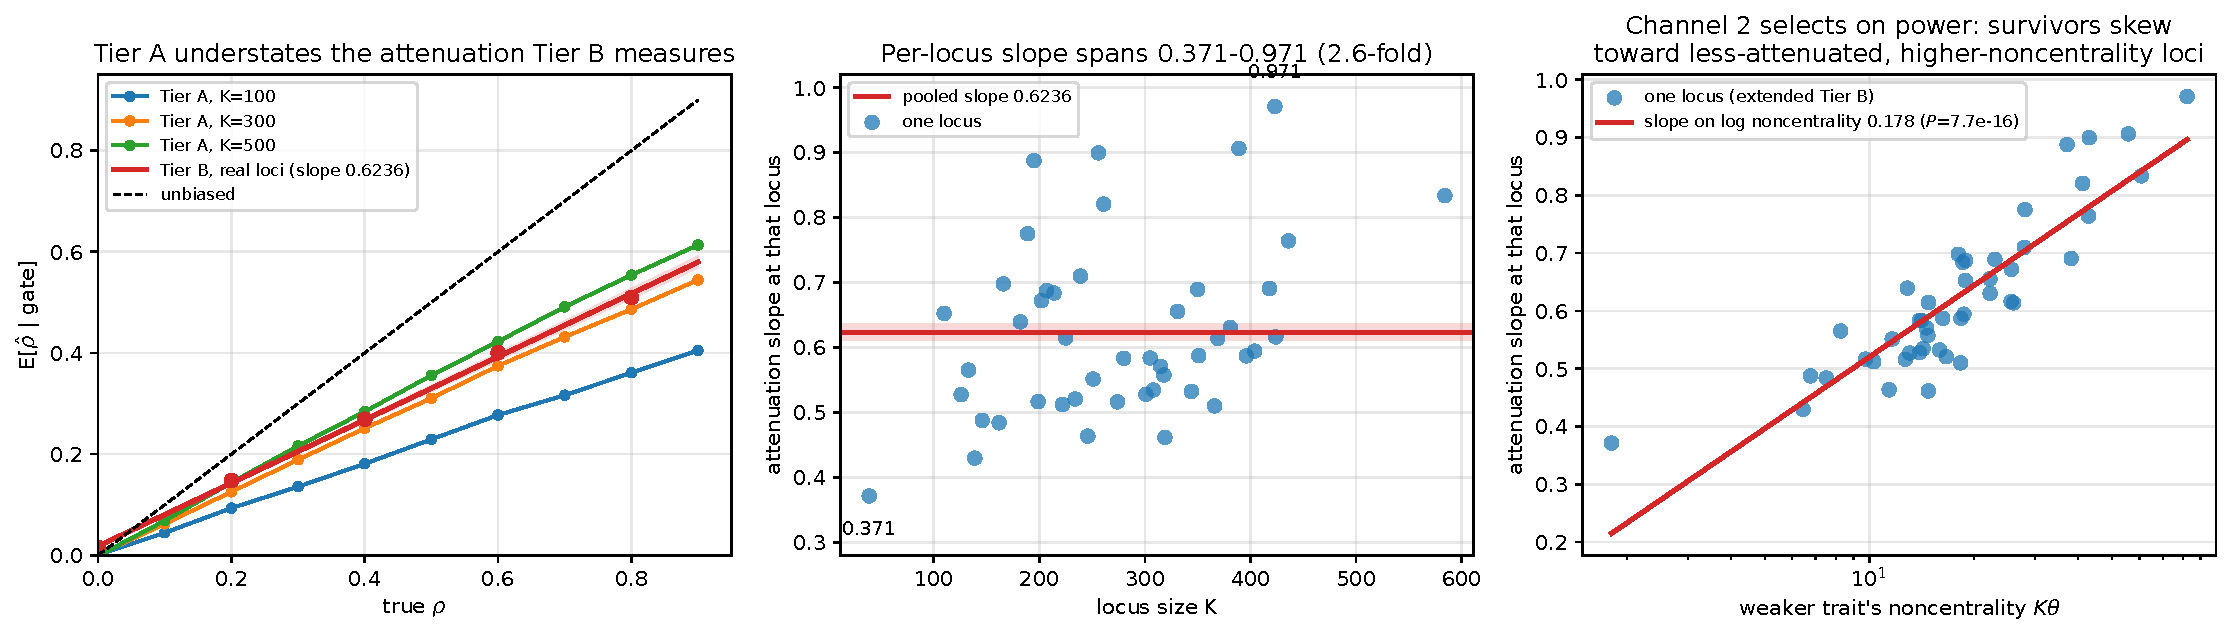
\includegraphics[width=0.95\textwidth]{Figure2_attenuation.pdf}
\caption{\textbf{The filter attenuates the estimates that survive it.} Reported $E[\rh\mid G]$ against true $\rho$ under Tier~A and Tier~B, the fitted per-locus slope against locus size $K$, and that slope against the weaker trait's noncentrality $K\theta$.}
\label{fig:2}
\end{center}
\end{figure}

\subsection{Overlap manufactures correlation, and a constant rule for it
fails}\label{sec:intercept}

At a true $\rho$ of zero the filter combined with sample overlap yields a non-zero
expected reported correlation. In Tier~A, holding $K=300$ and both heritabilities fixed
and varying only the overlap, the reported $\rh$ at $\rho=0$ rises from 0.0008 at $\re=0$
to 0.0340 at $\re=0.05$ and 0.0666 at $\re=0.10$, that is, linearly in $\re$ with intercept
$\approx0.68\,\re$; a held-out cell at $\re=0.20$, with its own $K$ and heritabilities,
reports 0.156. On P4 that rule works:
$\re=0.02756$ predicts 0.019 and Tier~B on 46 real loci observed 0.0182
($P=4.3\times10^{-7}$), a statistically significant correlation manufactured entirely out
of shared noise.

We pre-specified $0.68\,\re$ as the rule to be scored across the panel, but it failed by
a wide margin. It predicts 0.145 on P1 where Tier~B measures 0.028, and averaged over six
pairs its absolute error is 0.0432, which on a parameter bounded in $[-1,1]$ is not a
usable prediction. The constant was read
off Tier~A in a low-power configuration, but $\Ilocus\propto\Delta_i$ and $\Delta_i\to0$
as power grows, so the manufactured intercept must shrink for well-powered pairs, which
are exactly the pairs with the largest $\re$ in this panel. Evaluating the closed form on
each pair's own per-locus $(K,\theta_1,\theta_2,\re)$ reduces the mean absolute error from
0.0432 to 0.0050 (Table~\ref{tab:panelout}).

The replacement statement is conditional. Where the
filter binds, overlap manufactures correlation at a magnitude that can exceed published
local genetic correlations: 0.139 on P3, whose ASD and ADHD GWAS share the iPSYCH cohort.
Where it is close to non-binding the intercept is small almost regardless of $\re$: P1 has
the panel's largest overlap at $\re=0.214$ and one of its smallest intercepts at 0.028.
Overlap alone is insufficient for an analyst to know whether there is a problem, but
together with power it is informative enough. The P2 contrast exposed this as removing UK
Biobank did not lower the measured overlap ($0.1090\to0.1132$) but did lower power, and the
closed form tracks the resulting rise in both arms' intercepts because it is a function of
both jointly.

\subsection{Intervals are calibrated and nearly vacuous}\label{sec:intervals}

Post-filter coverage is 0.949 against a nominal 0.950, so the filter does not break
LAVA's intervals. Width is however a problem. Mean simulated post-filter width is 1.386 on
a parameter bounded in $[-1,1]$, spanning 69\% of the parameter space, and the simulation
predicts the real intervals closely without being fitted to them (1.365 observed on P4).
The fraction of simulated intervals excluding zero is 0.139 at $\rho=-0.4$ and 0.123 at
$\rho=+0.4$, so the count of sign-determinate loci cannot discriminate between hypotheses
about direction. On P4 every one of the ten determinate intervals
has its upper bound pinned at 1.000 by \texttt{cap.estimates}, so the sign is determined
while the magnitude is not.

\begin{figure}[htbp]
\begin{center}
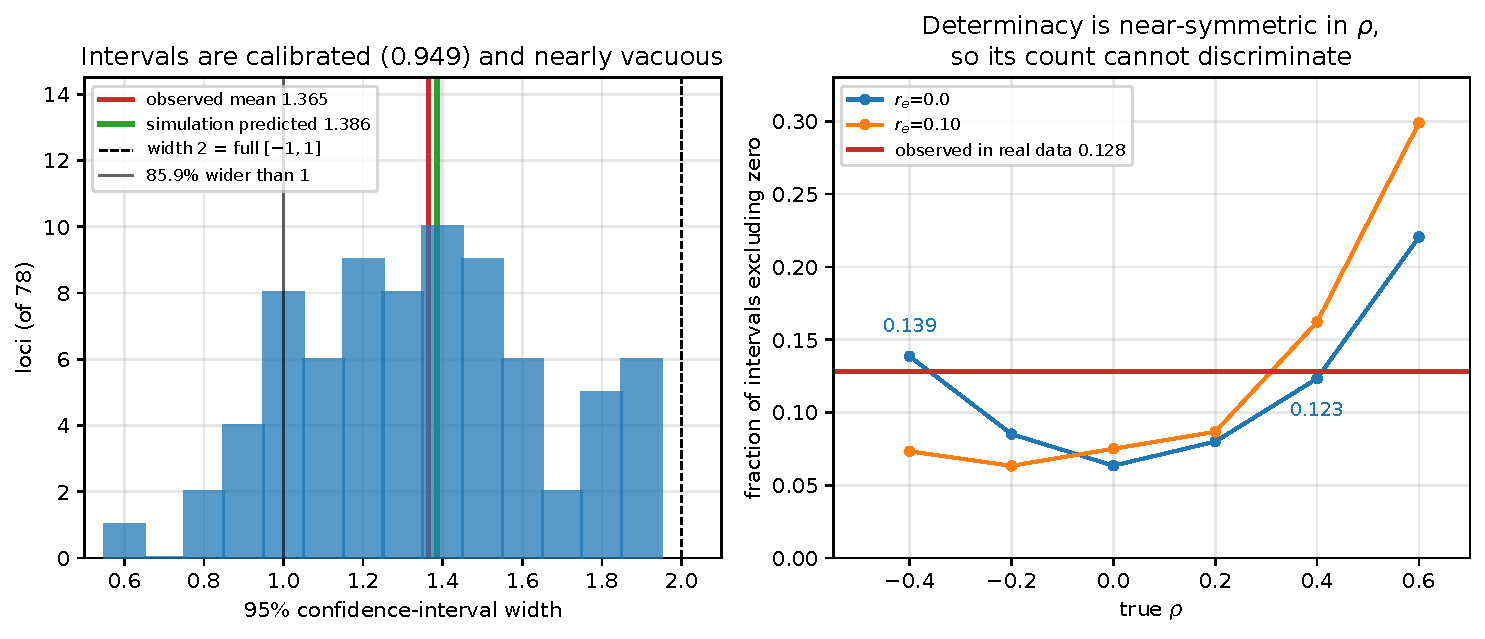
\includegraphics[width=0.95\textwidth]{Figure3_intervals.pdf}
\caption{\textbf{The intervals are correctly calibrated and nearly uninformative.} Distribution of 95\% confidence-interval width across P4's 78 reported loci, against the width-2 line that marks the whole parameter space, and the fraction of intervals excluding zero as a function of true $\rho$.}
\label{fig:3}
\end{center}
\end{figure}

\begin{figure}[htbp]
\begin{center}
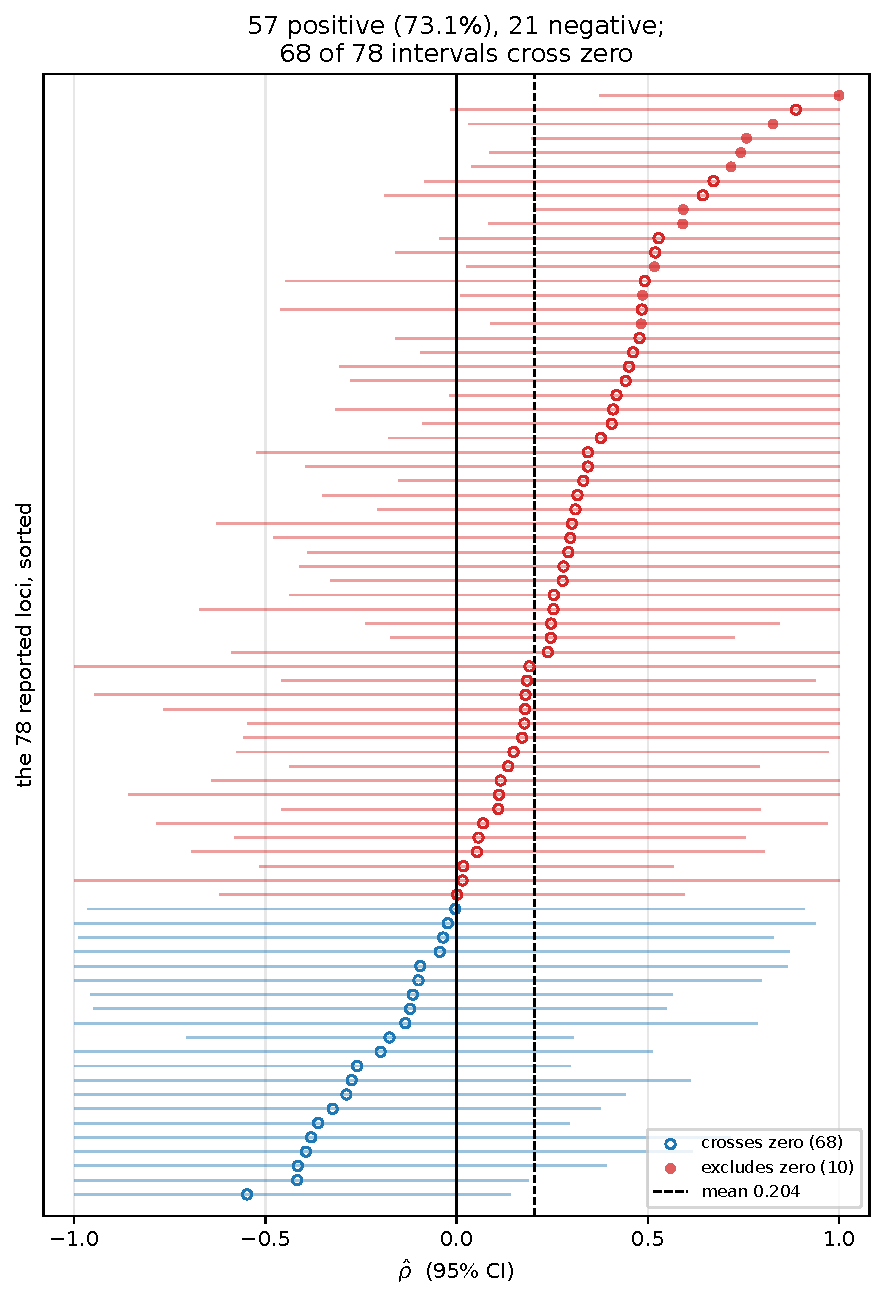
\includegraphics[width=0.95\textwidth]{Figure4_the_78_loci.pdf}
\caption{\textbf{All 78 reported local genetic correlations for P4, sorted.} Each row is one locus with its 95\% confidence interval, colored by sign; filled points are the 10 intervals excluding zero and open points the 68 crossing it.}
\label{fig:4}
\end{center}
\end{figure}

\subsection{The correction, and the penalty for applying it per
locus}\label{sec:corrperf}

Over 48 simulation cells the aggregate gate-aware correction reduces mean absolute bias
from 0.247 to 0.026, a factor of 9.7, and by a factor of 7.6 relative to a single pooled
factor (Table~\ref{tab:corr}).

The pooled factor uses the best available genome-wide slope, 0.6236, and performs worse
than the earlier and less accurate 0.5512 did (0.195 against 0.182). A single factor
fails to encapsulate the heterogeneity it is asked to summarise. A pooled factor is not an
approximation to the right answer that improves as the pooling improves, it is the wrong
shape of answer.

The per-locus variant is markedly worse than the aggregate one, 0.106 against 0.026,
because $g_K$ is nonlinear and floored. Correction also does not rescue per-locus
inference: the interval transforms by the same map, so its width scales by $1/\Slocus$,
between 1.95$\times$ and 3.01$\times$ across the validation cells. Applied to the observed
mean width of 1.365 that gives 2.27, wider than the entire parameter space. Correcting a
point estimate cannot narrow its interval, and the interval is the binding constraint on
any per-locus claim.

\begin{table}[htbp]
\caption{Correction performance over 48 simulation cells.}\label{tab:corr}
\small
\begin{center}
\begin{tabular}{@{}lrr@{}}
\toprule
Estimator & Mean abs.\ bias & Max abs.\ bias \\
\midrule
Uncorrected, as LAVA reports         & 0.247 & 0.602 \\
Single pooled factor ($\div$ 0.6236) & 0.195 & 0.579 \\
Gate-aware, applied per locus        & 0.106 & 0.304 \\
Gate-aware, applied in aggregate     & 0.026 & 0.107 \\
\bottomrule
\end{tabular}
\par\smallskip\footnotesize\noindent \textit{Note.} Bias is reported as the absolute difference between the mean estimate and the true $\rho$, averaged (mean) or maximized (max) over the 48 simulation cells.
\end{center}
\end{table}

\begin{figure}[htbp]
\begin{center}
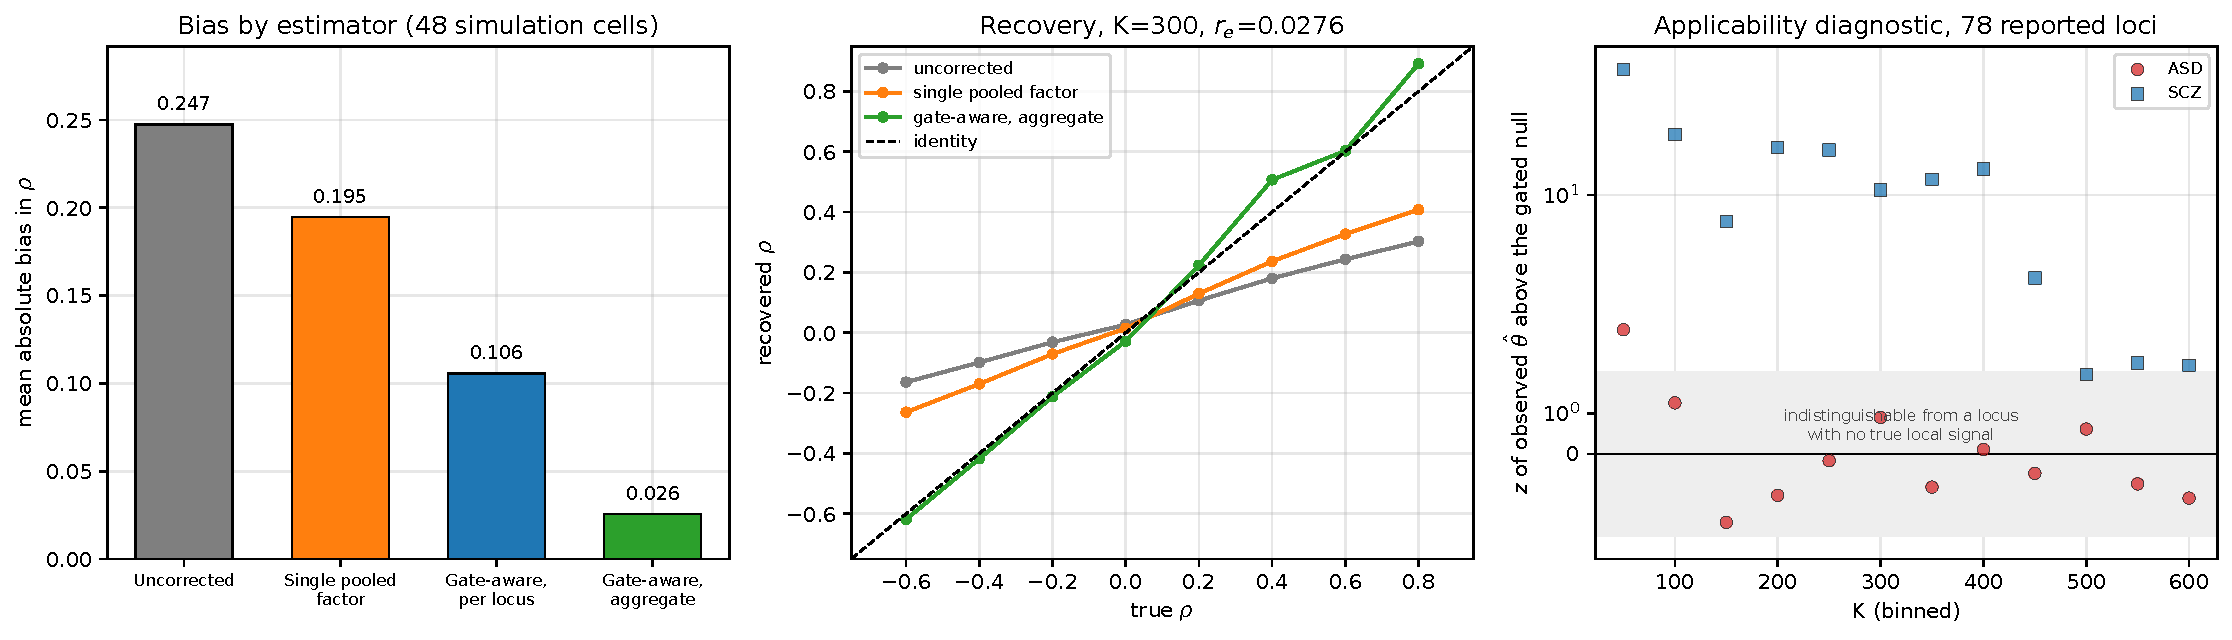
\includegraphics[width=0.95\textwidth]{Figure5_correction.pdf}
\caption{\textbf{The correction and its diagnostic.} Mean absolute bias and recovery of the true correlation under four estimators across the 48 validation cells, and the applicability diagnostic on real data by $K$ bin and trait, with the $\pm2$ band marking indistinguishability from a locus carrying no true local signal.}
\label{fig:5}
\end{center}
\end{figure}

\subsection{Three loci through the protocol}\label{sec:worked}

Three loci from P1, the panel's best-behaved pair, show the three cases the protocol has
to distinguish (Table~\ref{tab:worked}). At locus~A the weaker trait clears the filter but
not comfortably ($P=0.011$), so the gate is doing real selection work and the slope is
0.7217. The corrected estimate nonetheless moves only from 0.2588 to 0.2711, because at
$\re=0.2139$ the filter manufactures $+0.0632$ of apparent positive correlation here and
removing it before dividing all but cancels the inflation from dividing. A
practitioner who divided by the slope and forgot the intercept would report 0.359 instead
of 0.271, a 32\% overstatement, which is a likely way to misapply the
correction. At locus~B the correction is inert and should be, as both traits clear the
filter by orders of magnitude, the slope is 0.9881, and 0.4922 becomes 0.4916.

Locus~C cannot be corrected at all. Inverting $g_K$ returns $\theta_1=0$ exactly, so no
$\theta$ is consistent with the data other than the floor. This is not a rare edge case, as
353 of P1's 1,369 reporting loci (25.8\%) sit at the floor, in the pair that passes the
diagnostic most comfortably in the panel. A quarter of the elements do not exist, which is
the reason the correction is pooled.

\begin{table}[htbp]
\caption{Three P1 reporting loci taken through the correction;
$\re=0.2139$.}\label{tab:worked}
\small
\begin{center}
\begin{tabular}{@{}lrrr@{}}
\toprule
& A: loc.\ 874 & B: loc.\ 38 & C: loc.\ 168 \\
\midrule
Chromosome, $K$         & chr5, 357 & chr1, 285 & chr1, 345 \\
$P$, weaker trait       & 0.0114 & $1.78\times10^{-4}$ & 0.0310 \\
$P$, stronger trait     & $5.1\times10^{-11}$ & $1.34\times10^{-5}$ & $1.49\times10^{-5}$ \\
$\rh$ as reported       & 0.2588 & 0.4922 & $-0.6064$ \\
Recovered $\theta_1$    & 0.0800 & 0.3192 & 0.0000 \\
Recovered $\theta_2$    & 0.5660 & 0.3913 & 0.3509 \\
$\Slocus$               & 0.7217 & 0.9881 & --- \\
$\Ilocus$               & 0.0632 & 0.0064 & --- \\
At the selection floor? & No & No & Yes \\
$\rh_{\mathrm{corr}}$   & 0.2711 & 0.4916 & not identified \\
Interval width, after   & 1.3754 & 0.8656 & --- \\
\bottomrule
\end{tabular}
\par\smallskip\footnotesize\noindent \textit{Note.} $K$, principal components retained; $P$, univariate heritability $P$-value; $\theta_i$, local signal-to-noise ratio of trait $i$; $\Slocus$ and $\Ilocus$, per-locus attenuation slope and manufactured intercept; $\re$, sample-overlap correlation.
\end{center}
\end{table}

\subsection{The panel: attrition, prediction and diagnostic}\label{sec:panel}

All six pairs complete (Table~\ref{tab:panelout}). The rows carrying the most weight are
the closed-form and measured slopes, the only genuinely out-of-sample test in the paper:
the closed form is derived from a sampling model, while the measured value comes from
injecting a known $\rho$ into real loci and recovering it through LAVA's own code. The
largest discrepancy is 0.007 and the mean 0.0048, and the agreement holds across a slope
range of 0.579 to 0.923, from a regime where the filter destroys 42\% of the signal to
one where it costs 8\%, with no parameter fitted to the panel. That is what makes the
protocol usable. An analyst holding $K$, two univariate
$P$-values and an LDSC overlap estimate can compute the expected attenuation of their own
analysis before deciding whether to trust it.

The dominant loss is not the filter. On P4 the weaker trait's local variance estimate goes
negative at 1,429 of 2,400 processed loci (59.5\%) against 65 (2.7\%) for the stronger, due
to the undocumented Channel~2. While we had expected the filter to be the primary
constraint, the weaker trait sets the ceiling at every stage.

The diagnostic separates the panel cleanly. P5 reports 73 loci and P4 reports 78, while
accepted P2b reports 545, so the separation is not by effect size or locus count. It
detects whether the denominator carries signal at all. One correction to our own procedure
belongs here: C3 as frozen referred the conditional pass rate to a flat
$\alpha=0.05$ rather than to the conditional null $0.05/P(\chi^2_K\ge K)\approx0.103$, so
every value roughly doubles when recomputed. The 0.40 threshold falls between the two
groups under either baseline and all six verdicts are identical. We report both.

\begin{table}[htbp]
\caption{Protocol output across the panel. Closed-form slope and intercept are
$\Slocus$ and $\Ilocus$ evaluated on each pair's own per-locus
$(K,\theta_1,\theta_2,\re)$ and averaged over the loci Tier~B fitted; measured
values are that pair's extended Tier~B fit. C1--C3 are the diagnostic checks of
Section~\ref{sec:correction}, reported as frozen. Percentages for estimability and
Channel~2 loss are of processed blocks.}\label{tab:panelout}
\small
\begin{center}
\resizebox{\textwidth}{!}{%
\begin{tabular}{@{}lrrrrrr@{}}
\toprule
Quantity & P4 & P1 & P2a & P2b & P3 & P5 \\
\midrule
Blocks processed             & 2,400 & 2,487 & 2,483 & 2,483 & 2,424 & 2,458 \\
Weaker trait estimable       & 40.5\% & 95.3\% & 86.7\% & 74.4\% & 42.0\% & 40.0\% \\
Both estimable               & 37.8\% & 92.7\% & 83.9\% & 72.9\% & 40.3\% & 39.1\% \\
Reported loci                & 78 & 1,369 & 816 & 545 & 84 & 73 \\
Reported, \% of blocks       & 3.13 & 54.87 & 32.71 & 21.84 & 3.37 & 2.93 \\
Bonferroni survivors         & 0 & 98 & 20 & 8 & 0 & 0 \\
Channel~2 loss, weaker       & 59.5\% & 4.7\% & 13.3\% & 25.6\% & 58.0\% & 60.0\% \\
Channel~2 loss, stronger     & 2.7\% & 2.6\% & 3.1\% & 2.0\% & 1.7\% & 0.9\% \\
Median $K$                   & 268 & 295 & 290 & 290 & 229 & 223 \\
Measured $\re$               & 0.0276 & 0.2139 & 0.1090 & 0.1132 & 0.2372 & 0.0945 \\
\midrule
Slope, closed form           & 0.620 & 0.902 & 0.917 & 0.877 & 0.619 & 0.578 \\
Slope, measured (Tier~B)     & 0.624 & 0.908 & 0.923 & 0.882 & 0.612 & 0.579 \\
Intercept, closed form       & 0.0174 & 0.0360 & 0.0166 & 0.0249 & 0.1476 & 0.0696 \\
Intercept, measured          & 0.0182 & 0.0283 & 0.0125 & 0.0205 & 0.1389 & 0.0652 \\
Intercept, $0.68\,\re$ rule  & 0.0187 & 0.1454 & 0.0741 & 0.0770 & 0.1613 & 0.0643 \\
\midrule
C1, slope fold-change        & 2.66 & 1.02 & 1.03 & 1.08 & 2.87 & 4.70 \\
C2, pooled $z$, weaker trait & $-0.2$ & $+38.8$ & $+18.0$ & $+8.1$ & $-0.2$ & $-0.2$ \\
C3, null fraction, weaker    & 0.49 & 0.07 & 0.10 & 0.14 & 0.44 & 0.53 \\
Corrected magnitude usable?  & No & Yes & Yes & Yes & No & No \\
\bottomrule
\end{tabular}}
\par\smallskip\footnotesize\noindent \textit{Note.} P1--P5 are defined in Table~\ref{tab:panel}. C1, slope stability across $K$ strata (pass if $<1.25$); C2, distance of the weaker trait from the selection floor (pass if pooled $z\ge5$); C3, fraction of gate passes attributable to chance (pass if $\le0.40$).
\end{center}
\end{table}

\begin{figure}[htbp]
\begin{center}
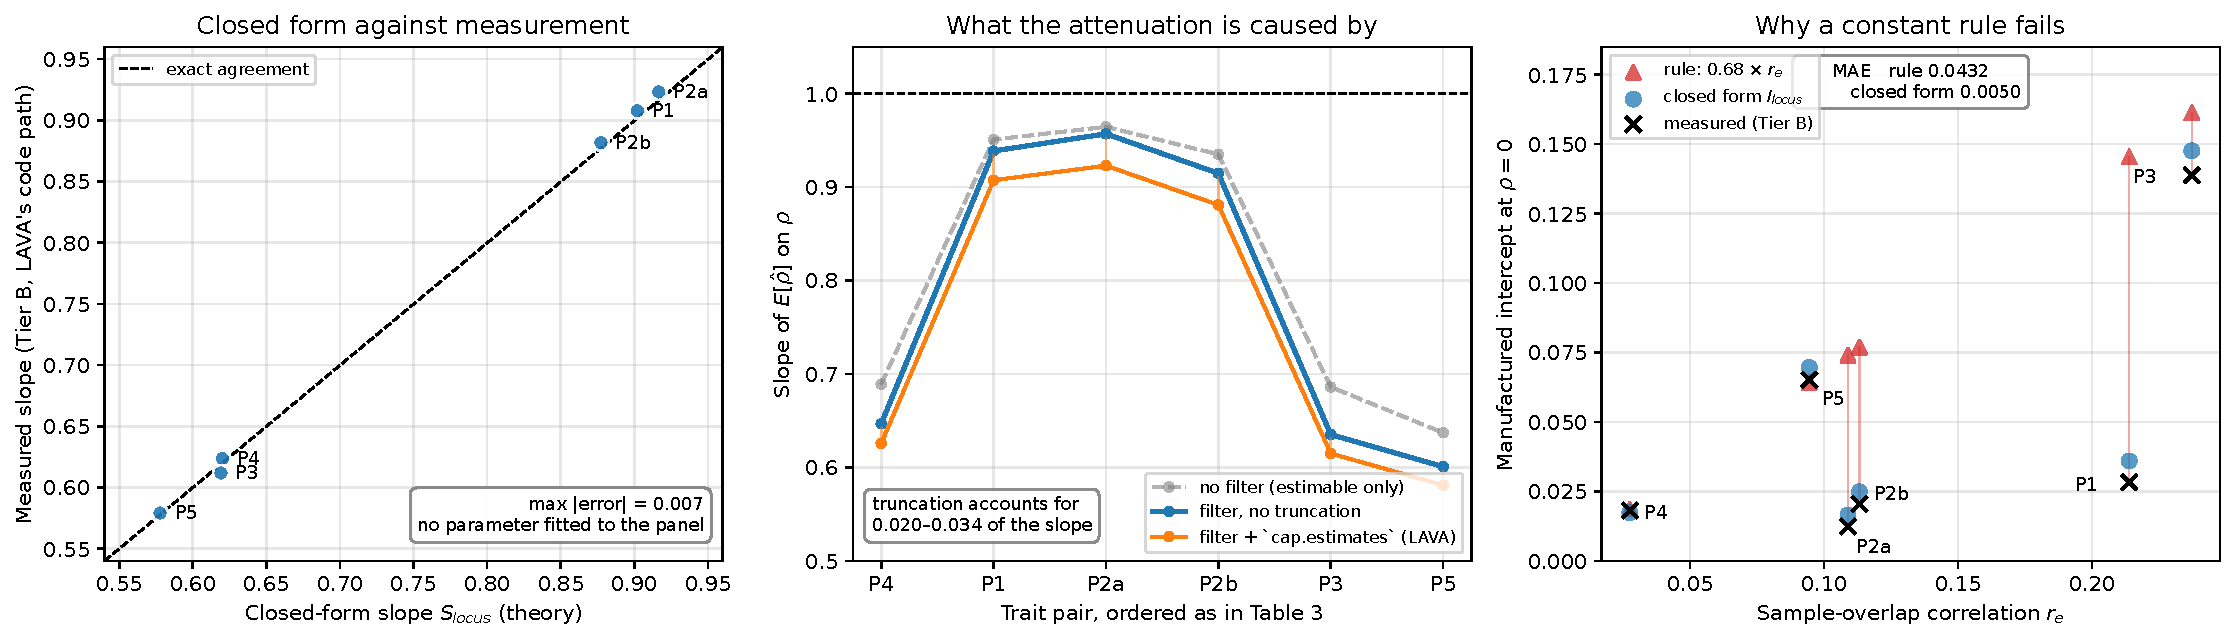
\includegraphics[width=0.95\textwidth]{Figure6_validation.pdf}
\caption{\textbf{Validation and attribution.} (a) The closed-form slope $\Slocus$ against the slope Tier~B measures on each pair's real loci, for all six pairs; (b) the attribution control of Table~\ref{tab:tierC}; (c) the manufactured intercept against $\re$, with the pre-specified $0.68\,\re$ rule, the closed form and the measurement.}
\label{fig:6}
\end{center}
\end{figure}

\subsection{A pair that fails the diagnostic, and what that
shows}\label{sec:failing}

P4 fails all three criteria, and the failure is instructive because it is the regime a
large fraction of psychiatric applications occupy. Across $K$ stratifications from 1 to 8
strata its aggregate slope moves from 0.769 to 0.288 and the implied corrected mean from
0.25 to 0.64. The floor diagnostic explains why. At the 78 reporting loci the weaker
trait's observed mean gated heritability is indistinguishable from what a locus with no
true local signal reports after passing the filter, at per-bin $z$ from $-1.67$ to $+3.05$
against $+1.95$ to $+48.3$ for the stronger trait.

A test that does not depend on the pass rate at all agrees, which is decisive.
Under a complete local null $p_i$ is uniform and Channel~2 retains exactly those loci with
$p_i\le q_i:=P(\chi^2_{K_i}\ge K_i)$, so $u_i=p_i/q_i$ is Uniform$(0,1)$ on the retained
loci. Across the weaker trait's 971 estimable loci that null is not
rejected: mean $u=0.491$ against 0.5, Kolmogorov--Smirnov $P=0.47$. The same trait gives
$P=0.078$ and $P=0.86$ in the two other pairs it appears in, while all nine remaining
trait-analyses in the panel reject at $P<10^{-120}$.

We conclude that within this analysis the weaker
trait carries no detectable local heritability signal anywhere in the genome, and the 78
reported loci are not a set of weak findings but what the filter emits when one of its two
inputs is noise. Taking them at face value compounds the error. 57 of 78 are positive,
which a binomial test against 50/50 returns at $P=5.6\times10^{-5}$, but 0.5 is not the
null when the two GWAS share samples, and the filtered null gives $P=3.8\times10^{-4}$.
Dividing such estimates by a genome-wide attenuation slope, the only correction
previously available, actively misleads, because the reporting loci are the high-power
tail where attenuation is mildest.

\section{Discussion}\label{sec:discussion}
%% =====================================================================

\subsection{Reporting guidance}\label{sec:guidance}

We suggest some guidance on reporting that users of LAVA, and of comparable tools, can
follow, each item traceable to a result.

\begin{enumerate}
\item \textbf{Report the attrition cascade, not only the reported loci}: how many blocks
  entered, how many were processed, how many were estimable per trait, and how many passed.
  A study reporting 78 loci without stating that the other 2,417 blocks returned no
  estimate misleads the reader into assuming that the genome was tested.
\item \textbf{Check for Channel~2 explicitly.} Verify that \texttt{process.locus()}
  returned both phenotypes before scoring the filter. Code that does not check this will
  report a comparison that was never made.
\item \textbf{Never correct with a single factor.} The slope varies from 0.371 to 0.971
  across real loci within one pair and from 0.579 to 0.923 between pairs. Compute $\Slocus$
  instead.
\item \textbf{Run the applicability diagnostic before reporting any corrected magnitude},
  and where observed gated heritability is not clear of the selection floor, report the
  uncorrected estimate with the attenuation stated as a bound.
\item \textbf{Report interval width alongside coverage, and do not test sign against
  50/50.} Coverage is fine, but width is the problem. Where the two GWAS share samples,
  the filtered null is shifted, so the naive test overstates significance.
\item \textbf{Compare conditional rates against conditional nulls.} A gate pass rate
  computed among loci that survived Channel~2 must be referred to
  $0.05/P(\chi^2_K\ge K)\approx0.103$, not to 0.05. We made this error ourselves.
\item \textbf{Report the phenotype set used to build the input object, and state $\re$
  without reading the manufactured intercept off it alone.} That composition sets the $K$
  cap and the common-SNP set, and the panel's highest-overlap pair ($\re=0.214$) has one of
  its smallest intercepts (0.028).
\end{enumerate}
\subsection{What this means for already published results, and how far it generalizes}\label{sec:published}

The correction consumes only $K$, two univariate $P$-values, $\rh$ with its interval, and
an overlap estimate, each printed in a typical LAVA supplementary table or recoverable
from one, so the protocol applies retrospectively without the original genotypes, the LD
reference, or the summary statistics. That was a design requirement, because the great
majority of local genetic correlations that will ever be interpreted have already been
published.

Most published estimates are probably fine, and this paper should not be read as saying
otherwise. Attenuation tracks the weaker trait's power and on the panel ranges from 8\% to
42\%. A study of two well-powered disorders with large $K$ is in P1's regime, where the
slope is 0.908 and the manufactured intercept 0.028 despite an $\re$ of 0.214. Its bias is a function of the analysis, is currently unreported, and is now computable. Where the weaker trait is
underpowered the magnitudes should be treated as lower bounds and the sign claims
re-examined, and that regime is recognizable without re-analysis: a large Channel~2 loss
rate for one trait, a small reporting fraction, and few or no Bonferroni survivors.

The closest classical relative is Berkson's admission artifact \citep[][]{ref14}, in which a
sample selected on a function of two variables acquires an association absent in the
population. The difference is that the selected variables here are the estimand's
denominator, so the induced dependence propagates into a ratio. That structure is not
specific to LAVA, and whether $\rho$-HESS, SUPERGNOVA and LOGODetect share it is a
question the benchmarking literature \citep{ref5} is well placed to answer and did not
ask.
\subsection{Limitations}\label{sec:limitations}

\begin{itemize}
\item \textbf{The attenuation slope is a lower bound, not a point estimate.} Tier~B can be
  fitted only on loci surviving Channel~2, which removes low-power loci, and enlarging the
  sample does not fix it, so no unbiased genome-wide slope is obtainable this way.
\item \textbf{A two-trait local genetic correlation is not reproducible from the trait
  pair alone.} \texttt{process.input()} reduces every phenotype to the SNPs common to all
  phenotypes in the object: analyzing ASD $\times$ SCZ inside an eight-phenotype object
  would have cut usable SNPs from 5,774,835 to 2,306,339. Since the slope depends strongly
  on $K$, the same two GWAS analyzed in a larger object return a more attenuated answer,
  and published estimates from multi-phenotype studies are not directly comparable to
  two-trait ones.
\item \textbf{The $\chi^2_K$ reference distribution is not exactly calibrated on these
  data, and we cannot fully explain the discrepancy.} A complete local null implies
  survival of Channel~2 at $P(\chi^2_K\ge K)\approx48.7\%$ of loci and real signal can only
  raise that figure, yet one trait sits below it in all three analyses it appears in
  (40.5\%, 42.0\%, 40.0\%). Verdicts are unaffected, but the absolute calibration of the
  floor quantities is approximate.
\item The derivation covers binary traits, since the $F$-test LAVA applies to continuous
  traits changes the selection geometry, and analyses are European-ancestry only, forced by
  the LD reference.
\item The second-order form is an approximation, though the discrepancy is at most 0.007
  against Tier~B, and the diagnostic is a necessary condition rather than a sufficient one:
  passing it only establishes that $\theta$ is identified, not that the sampling model holds.
\end{itemize}
\section{Conclusion}\label{sec:conclusion}

LAVA's univariate significance filter is a selection event on the denominator of a ratio
estimator, and the two are not separable: passing the filter implies a positive
denominator, and \texttt{run.bivar()} cannot run without one. The filter's effect is
available in closed form under LAVA's own sampling model, affine in the true
correlation, and computable per locus from quantities every run already reports. Across
six trait pairs that closed form predicts the measured attenuation slope to within 0.007,
with nothing fitted to the panel.

The size of the bias is a property of the analysis. Where the filter
binds the damage compounds: 42\% of the signal destroyed, per-locus slopes from 0.371 to
0.971 so that no single factor can correct it, an overlap-driven intercept manufacturing
significant correlation from shared noise, and intervals too wide to determine the sign at
87\% of the loci it reports (68 of 78 on P4). Where it does not bind, LAVA is close to unbiased and the correction here
close to unnecessary. That is itself worth reporting, because the alternative reading of an
uncharacterized filter is that every published estimate is suspect, and that is not what
we find. A study that reports filtered local genetic correlations without the attrition
cascade, the interval widths and, where sign is at issue, the filtered null is not
reporting a genome-wide test, but the small, power-selected window its weaker trait
permitted.


\section*{Acknowledgments}

The authors thank the Psychiatric Genomics Consortium and the contributing study
participants, whose summary statistics made this work possible. The authors also thank
Dr.\ Alex Becker for mentorship and guidance throughout this project.

\medskip
\noindent\textbf{Funding.} This work received no funding from any agency in the public,
commercial or not-for-profit sectors.

\section*{Conflict of interest}

The authors declare no competing interests.

\section*{Ethics statement}

This study used only previously published, publicly available aggregate GWAS summary
statistics. No individual-level data were accessed and no new participants were recruited.

\section*{Use of AI tools}

The authors used large language models to edit the text of this manuscript and to help
write the analysis code. No section of the text, and no figure, table or reference, was
taken from a model's output without the authors' own revision. All code was read and
checked by the authors, and every numeric claim in the manuscript is verified against its
source file by \texttt{code/python/16\_audit\_numbers.py}. The authors are responsible for
the whole of the content.

\section*{Data and code availability}

\noindent All analysis code, the correction module and every result file underlying a
number in this paper are deposited at \url{https://github.com/riddhimanjain/lava-gate} and
archived at Zenodo \citep{refdata} under the MIT license, at
\url{https://doi.org/10.5281/zenodo.22830134} for the version used here and
\url{https://doi.org/10.5281/zenodo.22132758} for all versions. The deposit is
self-contained: the verification and audit scripts of Sections~\ref{sec:tiers},
\ref{sec:attrib}, \ref{sec:intercept} and \ref{sec:failing} run from the deposited
\texttt{results/} directory alone, without the bulk data.

The correction and the applicability diagnostic are supplied as a dependency-free R module
(\texttt{code/R/lavagate.R}, base R $\ge$ 4.0) consuming LAVA's own output, so they can be
applied to previously published local genetic correlations without re-running any
analysis. Two tests are included and are intended to be run before the code is trusted.
\texttt{code/R/test\_lavagate.R} checks the R implementation against the Python one used
for this paper's numbers; they agree to $1.3\times10^{-12}$ on $\Delta$ and
$1.8\times10^{-15}$ on the slope and intercept over 500 parameter combinations spanning
$K\in[50,500]$, $\theta\in[0.005,0.30]$ and $\re\in[0,0.20]$, and it re-derives P4's
published aggregate slope, intercept and interval widths.
\texttt{code/python/14\_pair\_pipeline.py --selftest} checks that the generic per-pair
pipeline reproduces P4 to floating point, including its diagnostic verdict. Verification
is deposited as runnable code and as raw output under \texttt{results/verification/}:
\texttt{V0\_exactness\_check.R} (agreement with \texttt{run.univ()} and
\texttt{run.bivar()}, and the nesting of Section~\ref{sec:estimator}),
\texttt{V1\_gate\_attribution.R} (Table~\ref{tab:tierC}),
\texttt{V2\_gate\_null\_baseline.py} and \texttt{V3\_null\_calibration.py} (the conditional
null and the complete-null goodness of fit), \texttt{V4\_closedform\_vs\_tierB.py}
(Table~\ref{tab:panelout}) and \texttt{V5\_null\_recalibration.py} (the calibration
limitation of Section~\ref{sec:limitations}). V0 is a precondition for V1 and exits
non-zero if agreement is not exact. Every numeric claim in this manuscript is checked
against its source file by \texttt{code/python/16\_audit\_numbers.py}.

GWAS summary statistics are publicly available from the Psychiatric Genomics Consortium
(\url{https://pgc.unc.edu/for-researchers/download-results/}) and are documented with
accession details and download locations in \texttt{data/DATA\_SOURCES\_MULTIPAIR.md}
rather than redeposited. The LAVA LD reference panel (v1.1) and the 2,495-block genome
partition are distributed with LAVA. Reproducing the panel end to end additionally
requires those bulk files (approximately 16 GB). Software versions: LAVA 0.1.5, R 4.3.1,
Python 3.10.12, \texttt{numpy} 1.24.4, \texttt{scipy} 1.10.1.




\begin{thebibliography}{99}

\bibitem[{Berkson(1946)}]{ref14}
Berkson, J. (1946). Limitations of the application of fourfold table analysis to hospital data. \emph{Biometrics Bulletin}, \emph{2}, 47--53. \url{https://doi.org/10.2307/3002000}

\bibitem[{Bulik-Sullivan et al.(2015a)}]{ref7}
Bulik-Sullivan, B., Finucane, H. K., Anttila, V., et al. (2015a). An atlas of genetic correlations across human diseases and traits. \emph{Nature Genetics}, \emph{47}, 1236--1241. \url{https://doi.org/10.1038/ng.3406}

\bibitem[{Bulik-Sullivan et al.(2015b)}]{ref6}
Bulik-Sullivan, B. K., Loh, P.-R., Finucane, H. K., et al. (2015b). LD Score regression distinguishes confounding from polygenicity in genome-wide association studies. \emph{Nature Genetics}, \emph{47}, 291--295. \url{https://doi.org/10.1038/ng.3211}

\bibitem[{Demontis et al.(2023)}]{ref12}
Demontis, D., Walters, G. B., Athanasiadis, G., et al. (2023). Genome-wide analyses of ADHD identify 27 risk loci, refine the genetic architecture and implicate several cognitive domains. \emph{Nature Genetics}, \emph{55}, 198--208. \url{https://doi.org/10.1038/s41588-022-01285-8}

\bibitem[{Gerring et al.(2022)}]{ref2}
Gerring, Z. F., Thorp, J. G., Gamazon, E. R., \& Derks, E. M. (2022). A local genetic correlation analysis provides biological insights into the shared genetic architecture of psychiatric and substance use phenotypes. \emph{Biological Psychiatry}, \emph{92}, 583--591. \url{https://doi.org/10.1016/j.biopsych.2022.03.001}

\bibitem[{Grove et al.(2019)}]{ref8}
Grove, J., Ripke, S., Als, T. D., et al. (2019). Identification of common genetic risk variants for autism spectrum disorder. \emph{Nature Genetics}, \emph{51}, 431--444. \url{https://doi.org/10.1038/s41588-019-0344-8}

\bibitem[{Heckman(1979)}]{ref4}
Heckman, J. J. (1979). Sample selection bias as a specification error. \emph{Econometrica}, \emph{47}, 153--161. \url{https://doi.org/10.2307/1912352}

\bibitem[{Jain(2026)}]{refdata}
[dataset] Jain, R. (2026). \emph{lava-gate: Analysis code, results and correction module for local genetic correlation} [Data set and software]. Zenodo. \url{https://doi.org/10.5281/zenodo.22830134}

\bibitem[{Lee et al.(2011)}]{ref15}
Lee, S. H., Wray, N. R., Goddard, M. E., \& Visscher, P. M. (2011). Estimating missing heritability for disease from genome-wide association studies. \emph{The American Journal of Human Genetics}, \emph{88}, 294--305. \url{https://doi.org/10.1016/j.ajhg.2011.02.002}

\bibitem[{Mullins et al.(2021)}]{ref10}
Mullins, N., Forstner, A. J., O'Connell, K. S., et al. (2021). Genome-wide association study of more than 40,000 bipolar disorder cases provides new insights into the underlying biology. \emph{Nature Genetics}, \emph{53}, 817--829. \url{https://doi.org/10.1038/s41588-021-00857-4}

\bibitem[{Trubetskoy et al.(2022)}]{ref9}
Trubetskoy, V., Pardi{\~n}as, A. F., Qi, T., et al. (2022). Mapping genomic loci implicates genes and synaptic biology in schizophrenia. \emph{Nature}, \emph{604}, 502--508. \url{https://doi.org/10.1038/s41586-022-04434-5}

\bibitem[{Watson et al.(2019)}]{ref13}
Watson, H. J., Yilmaz, Z., Thornton, L. M., et al. (2019). Genome-wide association study identifies eight risk loci and implicates metabo-psychiatric origins for anorexia nervosa. \emph{Nature Genetics}, \emph{51}, 1207--1214. \url{https://doi.org/10.1038/s41588-019-0439-2}

\bibitem[{Werme et al.(2022)}]{ref1}
Werme, J., van der Sluis, S., Posthuma, D., \& de Leeuw, C. A. (2022). An integrated framework for local genetic correlation analysis. \emph{Nature Genetics}, \emph{54}, 274--282. \url{https://doi.org/10.1038/s41588-022-01017-y}

\bibitem[{Wray et al.(2018)}]{ref11}
Wray, N. R., Ripke, S., Mattheisen, M., et al. (2018). Genome-wide association analyses identify 44 risk variants and refine the genetic architecture of major depression. \emph{Nature Genetics}, \emph{50}, 668--681. \url{https://doi.org/10.1038/s41588-018-0090-3}

\bibitem[{Zhang et al.(2023)}]{ref5}
Zhang, C., Zhang, Y., Zhang, Y., \& Zhao, H. (2023). Benchmarking of local genetic correlation estimation methods using summary statistics from genome-wide association studies. \emph{Briefings in Bioinformatics}, \emph{24}, Article bbad407. \url{https://doi.org/10.1093/bib/bbad407}

\bibitem[{Z{\"o}llner \& Pritchard(2007)}]{ref3}
Z{\"o}llner, S., \& Pritchard, J. K. (2007). Overcoming the winner's curse: Estimating penetrance parameters from case-control data. \emph{The American Journal of Human Genetics}, \emph{80}, 605--615. \url{https://doi.org/10.1086/512821}

\end{thebibliography}


\section*{Supporting information}

Supporting information is provided as a separate file and contains Supplementary Methods
S1--S3, Supplementary Tables S1--S3 and Supplementary Figure S1.

\end{document}
